\chapter{Foundation}
\label{cha:foundation}

\section{Fingerprinting}
Web browser fingerprinting, also known as device fingerprinting, is the systematic collection of information to identify and later re-identify users. (\textcite{doty18}, p.3)(\textcite{amiunique})\\
This data tracking method works by obtaining data from the users web browser and using this data to create an unique fingerprint "hash". This hash is the key for later re-identifying the user. (\textcite{upi15}, p. 1)(\textcite{havens16}, p. 4)\\\\
With millions of computers and mobile devices in use and even more browsers, this identification method seems really unlikely to work at first sight. Nevertheless, it is an extremely reliable method for correlating data across websites or even web browsers with individual users. (\textcite{havens16}, p. 3)\\\\
Here is how it works:\\
There are currently over 7.5 billion people populating our planet. Imagine you have to identify a single person. By stating this specific person is male, you already cut the choice by half. Information about the ethnicity and age of this person as well as the time zone he lives in will narrow down the choice even more.\\
It's basically the same with web browser fingerprinting. The gender can be seen as an equivalent for the used operating system, the ethnicity as the browser and age as the browsers version. Information about the time zone and used language are easily acquirable by the browser and so are more specific details which help narrowing down the choice to nearly always one person.\\\\
This combination of properties can be obtained using code (time zone, screen resolution, plug-ins) and also be extracted from HTTP headers (user agent string). (\textcite{miele18}) \\\\
Web browser fingerprinting was first developed roughly before 2010 and due to its effectiveness quickly gained traction in the tracking industry.(\textcite{havens16}, p. 3) \\
Many of the fingerprinting methods can not be detected by the user and as it is extremely difficult for users to modify their web browsers in a way that they are less vulnerable to it (\textcite{amiunique})(\textcite{miele18}), makes it a dangerous tool for deanonymization attacks and maliciously-minded tracking programs. (\textcite{havens16}, p.3)\\
\begin{tcolorbox}
Example\\
Upon accessing a website, the fingerprinting script determines the users fingerprint and pushes it to a central data store. This data store is usually a shared data store which is used by multiple websites. So when the user accesses another website which also has access to this shared data store, the user will be recognized and the user profile can be updated. (\textcite{havens16}, p. 8)
\end{tcolorbox}

%\subsection{Entropy} - (\textcite{khan14})
\section{Utilisation}
\label{sec:utilisation}
In a study conducted in 2013 by Nikiforakis et al. they found that fingerprinting is a part of some of the most popular websites on the internet and that multiple hundred thousands of users are fingerprinted on a daily basis. (\textcite{nikiforakis13}, p.6) \\\\
The following paragraphs lists different ways in which fingerprinting can be utilized:\\\\
Constructive use
\begin{itemize}
	\item Security authentication\\
	Using web browser fingerprinting to correctly identify a device which is used to log into an account can be used to re-identify a user and help combat fraud or credential hijacking. (\textcite{upi15}, p.4)(\textcite{nikiforakis13}, p.2)
	\begin{tcolorbox}
	Example:\\
	Services can track the devices used to access an account and inform the user in case an unknown device tries to access it. 
	\end{tcolorbox}
\end{itemize}
Destructive use
\begin{itemize}
	\item Hacking\\
	Habits of users can be tracked without their knowledge and attackers can acquire specific knowledge about the user’s software setup. (\textcite{upi15}, p.4) 
	\begin{tcolorbox}
	Example:\\
	With the help of web browser fingerprinting a hacker can acquire knowledge about the users operating system and adjust his hacking method accordingly.
	\end{tcolorbox}
\end{itemize}
Con- and destructive use
\begin{itemize}
	\item Identifying criminals\\
	As a mean of tracking, fingerprinting can be used to track people or even criminals. But as seen in the previous examples this can used for and against users. 
	\begin{tcolorbox}
	Example: positive use\\
	When a user is harassed or stalked by another user the website can use web browser fingerprinting as a mean of blacklisting said user. 
	\end{tcolorbox}
	\begin{tcolorbox}
	Example: negative use\\
	Citizens of countries with a strict regime can be blacklisted for expressing criticism against the government.
	\end{tcolorbox}
	\item Commercial use\\
	Commercial Fingerprinting is used to track people’s habits and preferences. The acquired knowledge can be used to either help the user or direct him into a certain direction. 
	\begin{tcolorbox}
	Example: positive use\\
	A website picks up the user’s habit to look for climbing gear and suggests similar products.
	\end{tcolorbox}
	\begin{tcolorbox}
	Example: negative use\\
	A website registers that the user recently bought more expensive products and starts to only show items in this certain price range rather than more suitable but cheaper products.
	\end{tcolorbox}
\end{itemize}
The following paragraphs will summarize the findings of a study conducted by Nikiforakis et al. in cooperation with three commercial fingerprinting companies in order to test multiple websites for the use of fingerprinting scripts.\\\\
Nikiforakis et al. used the categorization of TrendMicro and McAfee on a list of 3804 domains. If a domain was neither analysed nor categorized by the both used services they were marked as untested and not used. Therefore only 59.2\% of the 3804 domains were included in the results of this testing. If one service declared a domain as unsafe and the other stated the opposite, it was accepted as safe. Some categories were given aliases and gathered together to a more generalized category.(\textcite{nikiforakis13}, pp.6)\\\\
\begin{figure}[H]
\centering
		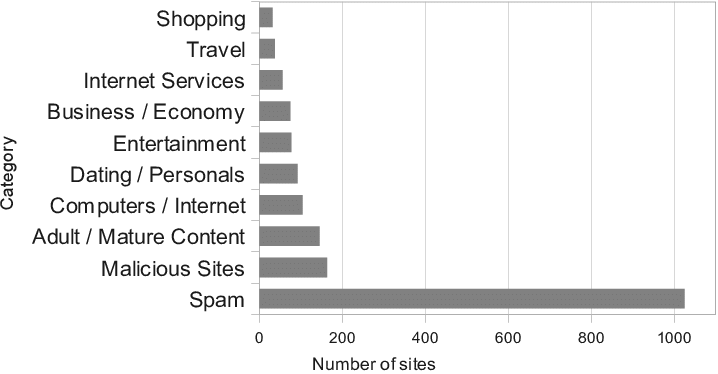
\includegraphics[width=350pt, height=160pt]{Top10CategoriesNiki.png}
		\caption{Top 10 categories utilizing fingerprinting (\textcite{Top10Niki})}
		\label{Top10Niki}
\end{figure}
This figure shows 10 categories, 8 of which operate with user subscriptions. These sites usually are interested in preventing hijacking of user accounts and fraudulent activities.\\
The top two categories were identified as malicious (163 domains) or as spam (1063 domains). Nikiforakis et al. noticed that many domains belonging to one of these categories were parked websites which do not include any fingerprinting code. Further many "quiz" or "survey" websites were located which in a later step extract a user's personal details. The domains were categorized as malicious if they exploit vulnerable browsers or extract private data from users.\\\\
It was discovered that all these sites were found to include, as some point, fingerprinting code provided by one of the three commercial fingerprinting companies.\\
This observation, paired with the fact that all of these three studied providers stated that there must be set an appointment in order to acquire fingerprinting services, point to the possibility that fingerprinting companies work with dubious domains in order to expand their fingerprinting database.(\textcite{nikiforakis13}, p.7)


\section{Threat}
have a look at (\textcite{eckersley10})

As seen in the previous sub-chapter /ref{sec:utilisation} web browser fingerprinting does have its advantages as well as its disadvantages for the user. This section will have a closer look as the threat fingerprinting poses for the users privacy.
 
Web browser fingerprinting is a tracking method, which can correlate user's browsing activity within as well as across sessions without transparency or control. (\textcite{doty18}, p.3) Most fingerprinting techniques are obscure and users usually don't notice that they are being tracked.

The modern web exposes a number of details about the user’s device, either directly or discoverable through testing. This is largely a result of a greater need to comply with different device types, support for different features, or simply leaking data by including too much information in protocol requests.
(\textcite{havens16}, p. 4)
 
Privacy and security

\begin{itemize}
	\item Identify a user: concerns about surveillance, personal physical safety, concerns about discrimination against them based on what they read or write when using the web. (\textcite{doty18}, p.4)
	\item An online party can correlate multiple visits (on same or different sites) to develop a profile or history of the user. This may occur without the user’s knowledge or consent and tools such as clearing cookies do not prevent further correlation. Also allows tracking across origins – different sites may be able to combine information about a single user even where a cookie policy would block accessing of cookies between origins. (\textcite{doty18}, p.4)
	\item Tracking without transparency or user control: bf allows for collection of data about user activity without clear indications that such collection is happening. Allows for tracking of activity without clear or effective user controls. (typically cannot be cleared or re-set) /*like cookies*/ (\textcite{doty18}, p.4f)
\end{itemize}

\textbf{go to original source}
High risk: 
In 2010 Peter Eckersley, in association with the Electronic Frontier Foundation(EFF), conducted a study of browser fingerprinting techniques. –
**	Group of people, expected to have high awareness of privacy concerns. 
**	Out of 470,161 browsers – 93,6% instantaneously unique finerprint
**	Group -> privacy-conscious users, informed of the dangers of browser fingerprinting
**	Simple algorithm for detecting changes in fingerprints.
o	Check to see if there is any fingerprint which, aside from one non-matching field, is otherwise the same.
o	Not make guess if there were multiple potential matches
o	Made 65,56\% guesses – 99,1% right
(\textcite{havens16}, p.6f)

**	Deanonymization of Tor users
Tor enables JavaScript by default and if the user fails to turn it off, even Tor users can be tracked due to the information leaked by JavaScript. (\textcite{havens16}, p.9f)

\subsection{Under General Data Protection Regulation}
This threat posed by web browser fingerprinting as depicted above might be reduced by the \textit{General Data Protection Regulation (GDPR)}, which entered into force on May 25th 2018. This regulation imposed by the European Union (EU) intends to cover exactly this kind of hidden data collection which is used by web browser fingerprinting, by forcing companies to prove they have a legitimate reason for the utilization of any means of tracking.(\textcite{miele18})\\\\
Even though the GDPR avoids specifying technologies it provides general rules which should keep up with technological development. Due to this regulation browser characteristics are now to be treated like personal data. Personal data has a broad definition as any information that might be linked to an identifiable individual can be passed as such. Examples for such are not only the IP-Address and MAC-Address of users but also less specific features, including the combination of characteristics which web browser fingerprinting relies upon. (\textcite{miele18})\\\\
In order to be allowed to use fingerprinting legally the concerned entity has to complete the following steps:\\
\begin{itemize}
	\item show that the tracking does not violate "the fundamental rights and freedoms of the data subject, including privacy", 
	\item and is in line with "reasonable expectations of data subjects"
	\item further give a legitimate argument for its interest in tracking,
	\item and share details about the scope, purposes, and legal basis of the data processing with the person subjected to the fingerprinting\\
\end{itemize}
Due to this regulation, the only step the user has to take to avoid fingerprinting is to say "no".\\\\
Even though the rules imposed by this regulation seem to help prevent unwanted tracking, it only helps mitigate it. There will certainly be fewer entities making use of fingerprinting though web browser fingerprinting is not expected to disappear, no matter how high the penalties are on its illegal utilisation.\\
Anyway, the GDPR only applies on processed personal data of individuals living in the \textit{European Economic Area (EEA)} for commercial purposes, or for any purposes when the behaviour is within the EEA. There will always be companies which either think they can escape the consequences or which claim to have "legitimate interest" in tracking users. Further, no matter how strict regulations are, it always comes down to the user. Due to the plentiful requests for consent as they are found on the web nowadays many users are worn out and do not take a second look at the privacy policy regulated by the GDPR. (\textcite{miele18})

\section{Mitigation}
As seen in the previous chapters there are many ways of utilizing web browser fingerprinting. Many of these possible applications pose a threat to the users privacy. So this brings up the question if there is a way to avoid this tracking method. Each of the researched articles about this topic stated the same. No. Unfortunately, there is no way to avoid being fingerprinted completely. There are only ways to try and reduce the risk of being tracked. (\textcite{web17})
The danger of web browser fingerprinting lays in its stateless nature. 
* hard to detect - if even possible
* impossible to opt-out
(\textcite{upi15}, p.4)
 \\\\
 \subsection{Best practice}
According to N. Doty (\textcite{doty18}, p.5), these are the best practices to mitigate the fingerprint we leave online: 
\begin{itemize}
	\item Avoid unnecessary or severe increases to fingerprinting surface
	\item Mark features that contribute to fingerprintability
	\item Specify orderings and non-functional differences
	\item Design APIs to access only the entropy necessary
	\item Enable graceful degradation for privacy-conscious users or implementers
	\item Avoid unnecessary new local state mechanisms
	\item Highlight any local state mechanisms to enable simultaneous clearing
	\item Limit permanent or persistent state\\
\end{itemize}
Further Doty mentions that this helps: 
\begin{itemize}
	\item Decreasing fingerprinting surface
	\item Increasing anonymity set
	\item detectable fingerprinting
	\item clearable local state
\end{itemize}
(\textcite{doty18}, p.7)\\

\subsection{Prevention?}
While N. Doty only listed ways to decrease the chance of being fingerprinted, R. Upathilake suggests the following steps to actually prevent the chance of being tracked via web browser fingerprinting (\textcite{upi15}, p.4):
\begin{itemize}
	\item Having all browser vendors agree on a single set of API calls to expose to the web applica-tions as well as internal implementation specifics;
	\item Having blocking tools which are maintained by doing regular web-crawls to detect tracking and incorporate blocking mechanisms into the tool;
	\item The introduction of a universal font list that a browser is limited to choose from for render-ing;
	\item Reporting unified and uncommunicative attributes
	\item Blocking or disabling js;
	\item Reducing the verbosity of the User-Agent string and the plug-in version;
	\item 	Having flash provide less system information and report only a standard set of fonts \\
\end{itemize}

\subsection{Canvas fingerprinting}
Is a difficult technique to automatically detect and prevent without false positives. A solution would be to turn to crowd-sourcing (sugg. By Acal et al.). A browser tool can de-fault to blocking all pixel data extraction attempts, but slowly over time, take into account user feedback and improve thetool to identify valid fingerprinting attempts. Other suggest-ed methods – having the browser add random pixel noise whenever pixels are extracted or having the browsers render scenes in a generic software renderer. These suggestions com e with a significant performance penalty and therefore, unacceptable for general use. The easiest method appears to require user approval if a script requests pixel data. Modern browsers already use this approach, for example with the html5 geolocation api. However, this introduces another permission dialogue which requires user interaction.
(\textcite{upi15}, p.4)

-- using private browsing modes or tor anonymity service
-- tor -> slower, less attrackive browsing experience
-- torbutton disables WebGL - still allows rendering to a <canvas> -> still partly vulnerable to canvas FP
-- mainstream users -> fingerprinting unavoidable consequence
(\textcite{mowery12}, p.1)


-- increasing the noise, but degrades the performance of <canvas> significantly for legitimate applications
-- same noise on multiple runs -> aid fingerprinting
-- therefore adding noise - not a feasible defence
-- one way would be: browser vendors - agree on a list of "canvas-safe" fonts
-- to support WebGL, ignore graphics card and render scenes in a generic software renderer
-- approach might be acceptable - performance impact not
-- easiest efficient defense: require user approval whenever a script requests pixel data 
-- modern browsers already implement this type for e.g. HTML5 geolocation APIs
(\textcite{mowery12}, p.10)

\subsection{Extensions and plug-ins}
The use of some common extensions and plug-ins were also mentioned in the liter-ature. The notable ones which seemed to aid in reducing fingerprintability were AdBlock Plus, Ghostery and NoScript. Nikiforakis et al. examined several highly rated extensions for firefox and chrome, which allowed changing the user-agent to appear as if sessions were from different computers. They noted in their study that these were inadequate and con-tained discrepancies which led to the browser being more distinguishable. These discrep-ancies allow fingerprinting scripts to increase the accuracy of the fingerprint since they are able to tell the presence of a specific extension. It should be noted that these results seem to be different from what was concluded by Yen et al. in their study. They suggested that changing the User-Agent string to one that corresponds to a populare browser version was a simple method to become less distinguishable. 
(\textcite{upi15}, p.4)

\subsection{The simplest solution}

-- browser extension -> automatically blocks active content e.g. JavaScript, Flash, or Silverlight applications (which don't deliver logically info to server)
-- these plugins - incl. NoScript (Firefox), ScriptBlock (Chrome) -> protection against canvas fingerprinting
-- using these plug-ins -> some web services or at least individual content -> stop working
-- not helpful if not sure if provider is trustworthy or not
-- these blockers can be directly used for fingerprinting the user
-- apart form script blocking solution
-- commonly-used browser and default settings
-- same with OS
-- high chance - no unique fingerprint and will be harder to track
(\textcite{web17})



\newpage
\section{Critical configurations and plug-ins}


https://www.1and1.ca/digitalguide/online-marketing/web-analytics/browser-fingerprints-tracking-without-cookies/

\begin{figure}
	\centering
	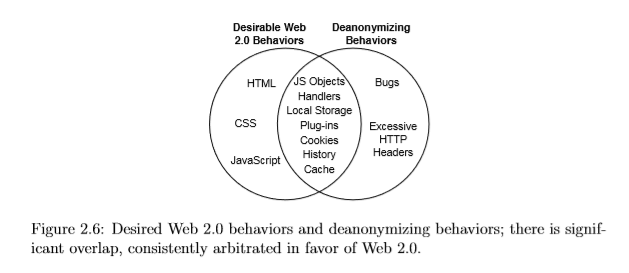
\includegraphics[width=0.7\linewidth]{images/dangerousConfigs}
	\caption{}
	\label{fig:dangerousconfigs}
\end{figure}
(\textcite{mayer09}, p.43)

As mentioned in the previous paragraph (chapter 2.1.) the scripts which use fingerprinting can read certain data via configuration settings or other observable characteristics from the web browser which enables them to create a specific fingerprint. (\textcite{doty18}, p.3)

The following paragraphs will introduce some of these certain information sources disclosed to third parties by the web browser and why they are used at all.


The information that browser fingerprinting reveals typically includes a mixture of HTTP headers (which are delivered as a normal part of every web request) and properties that can be learned about the browser using JavaScript code: your time zone, system fonts, screen resolution, which plugins you have installed, and what platform your browser is running on. Sites can even use techniques such as canvas or WebGL fingerprinting to gain insight into your hardware configuration.(\textcite{miele18})

\subsection{JavaScript}\label{JS}

JavaScript is enabled by default in all major browsers and by November 2018 JavaScript was included by 95\% of all websites online. (\textcite{w3techs18}).
-- therefore very useful tool - also because can query!
Js – the language which never works – for the developer

-- what is sputnik and test 262 ()

JS gives access to many browser-populated features like the plugins installed on the user’s device (\textcite{amiunique})

Identifying web browsers based on the underlying javascript engine
(\textcite{mulazzani13})

When JavaScript is disabled, websites won’t be able to detect the list of active plugins and fonts you use, and they also won’t be able to install certain cookies on your browser.
The disadvantage of disabling JavaScript is that websites won’t always function properly, be-cause it’s also used to make websites run smoothly on your device. This will impact your browsing experience.(\textcite{pixel18})

Browser fingerprinting, while a powerful tool, is often part of a larger suite of tracking techniques. Fingerprinting operates through the js engine as part of an analytics program. Any website that runs the fingerprinting analytics script will be able to track users through a shared data store.
(\textcite{havens16}, p.8)


Javascript has been standardized as ECMAScript [8],
and all major browsers implement it in order to allow
client-side scripting and dynamic websites. Traditionally,
Web developers use the UserAgent string or the navigator
object (i.e., navigator.UserAgent) to identify the client’s
Web browser, and load corresponding features or CSS files.
The UserAgent string is defined in RFC2616 [11] as a
sequence of product tokens and identifies the software as
well as significant subparts. Tokens are listed in order of their
significance by convention. The navigator object contains the
same string as the UserAgent string. However, both are by
no means security features, and can be set arbitrarily by the
user.
(\textcite{mulazzani13}, p.2)\\

SEE NIKIFORAKIS!!!!


\subsubsection{WebGL}\label{webgl}
%WebGL provides a JavaScript API for rendering 3D graphics in a <canvas> element. Modeled after OpenGL ES 2.0, WebGL is currently a draft specification and implemented and enabled in Chrome, Firefox, and Opera, as well as implemented but disabled in Safari. Each of these browsers provides a hardware-accelerated implementation, using the installed graphics hardware to render each frame. To mitigate serious misbehaviour and crashes, all of these browsers enable WebGL only for a whitelisted set of graphics cards and drivers.
%Current WebGL implementations expose their functionality through a separate canvas context (which will eventually be named “webgl”). The WebGL API is too complex to describe here in sufficient detail, but is stylistically similar to the desktop OpenGL API. It provides for vertex and fragment shaders, written in OpenGL Shading Language (GLSL), that, after compilation, run directly on the graphics card. WebGL also provides for OpenGL-style textures, as well as different lighting primitives. More advanced techniques, such as specular highlighting, bump mapping, and transparency, can be achieved through custom GLSL shaders. 2.4 SecurityImplications 
%(\textcite{mowery12}, p.3)


\subsection{Adobe Flash}\label{adobe}
Adobe Flash is a browser plug-in which provides different ways of delivering rich media content which could traditionally not be displayed using HTML. (\textcite{nikiforakis13}, p.3)


**	Criticized for poor performance, lack of stability
**	Newer technologies (HTML5) can potentially deliver what used to be only possible through flash – still available on the vast majority of desktops (\textcite{nikiforakis13}, p.3)
**	Returns all fonts with one simple call (\textcite{havens16}, p.5)
**	Its rich programming interface (API) provides access to many system-specific attributes (version of OS, list of fonts, screen resolution, timezone) (\textcite{amiunique})
**	Can be disabled without a negative impact on UEX – only impacts browsing experience on old websites(\textcite{pixel18}.)
**	Vulnerability, called “local storage objects” -> enables “zombie cookie” or “supercookie”. Almost impossible to remove. Populate numerous different storage areas with tracking in-formation. Even if cookies deleted from browser -> still come back. Other storage locations repopulate cookie as long as any existis – combined with brower fingerprinting, the cookies can track changes in fingerprints while also relying upon the fingerprint as a finale line of defense against the most privacy-conscious users. “cookie syncing” (\textcite{havens16}, p.8f)

SEE NIKIFORAKIS!!!!

\subsection{HTML 5 /Canvas}\label{html5}
-- HTML5 is the coding language used to build websites -> core fundamentals of every website
-- has the element "canvas"
-- originally html <canvas> element was used to draw graphics on a web page
(\textcite{pixel18})

Through the display of an HTML5 Canvas element, it is possible to collect small differences in the hardware on in the software configurations, thanks to slight differences in the image rendering between devices. The smallest pixel difference can be detected -> canvas fingerprinting 
(\textcite{amiunique})

%One of the most interesting new elements in HTML5, <canvas> provides an area of the screen which can be drawn upon programmatically. It enjoys widespread support, being available in the most recent versions of Chrome, Firefox, Internet Explorer, Opera, and Safari as well as Mobile Safari and Android Browser. The basic approach to drawing on a canvas is simple: acquire a graphics context, and use the context’s API to effect your changes. In the current HTML5 specification, the only defined context is“2d”. The 2d context provides basic drawing primitives such as fillRect, lineTo, and arc, as well as more complicated features such as B´ezier curves, color gradients, and copying in an existing image. 
%
%\textbf{refer to canvas fingerprinting}
%pixel extraction: In order for <canvas> to be a useful fingerprint, there must be some way to examine its behavior. Fortunately, <canvas> makes this extremely easy, providing several ways to inspect its data with pixel accuracy.
%(\textcite{mowery12}, p.2)
%
%First, the 2d context provides the method getImageData(). Given a rectangular region of the canvas, this method returns an ImageData object. Contained in this object are the RGBA values (as integers) for every pixel in the requested region. Second, the canvas object itself provides a toDataURL(type) method. When passed “image/png”, this method returns a data url consisting of the Base64 encoding of a PNG image containing the entire contents of the canvas. As this is a very convenient canvas-level method, we used this approach to extract data in our experiments. During black-box use of these fingerprints, the test suite could simply hash these data URLs, thereby removing the need to upload entire images from each client. It is worthwhile to note that these methods do preserve the same origin policy — if an image from a different origin has been drawn on this canvas, they will throw a SecurityError exception instead of returning pixel data. Therefore, our <canvas> fingerprints must only contain image resources that are under our control. 
%(\textcite{mowery12}, p.3)

\subsection{User agent}\label{UAS}
A user agent is a request header field in the hypertext transfer protocol (http) which is used for the communication between browser and website. (\textcite{xovi18}) It is automatically sent with each page call (\textcite{doty18}, p.6), except if it is specifically configured not to. (\textcite{xovi18})(\textcite{fielding14}, p.5.5.3)\\\\
The user agent contains the name and version of the used browser. In R. Fieldings work about http, this combination is also called product identifier. The product identifiers are listed in the order or their importance, whereas each of them can be followed by one or multiple comments. (\textcite{xovi18})(\textcite{fielding14}, p.5.5.3) This field value is often called user agent string. (\textcite{hoffman16})\\
\begin{tcolorbox}
Example 1: \\
Mozilla/5.0 (Windows NT 10.0; WOW64) AppleWebKit/537.36 (KHTML, like Gecko) Chrome/69.0.3497.102 Safari/537.36 Vivaldi/2.0.1309.37
\end{tcolorbox}
This string tells the receiving server, that the latest version (2.0.1309.37) of the Vivalid browser is used. In the comments (contained in the brackets) it gives away that the computer runs Windows 10 (Windows NT 10.0) on a 64-bit version (WOW64).\\
\begin{tcolorbox}
Example 2:\\
Mozilla/5.0 (Windows NT 10.0; Win64; x64) AppleWebKit/537.36 (KHTML, like Gecko) Chrome/64.0.3282.140 Safari/537.36 Edge/17.17134\\
\end{tcolorbox}
As well as with the other example, this browser (Edge with the version number 17.17134) also gives away the operating system and its version (same as before).\\\\
As shown in the examples above, not only the used browser name and its version are passed on but also information about the operating system and sometimes hardware. (\textcite{hoffman16}) (\textcite{xovi18}) The passed-on information is used to display different content in different browsers, on different oper-ating systems, or to gather statics (\textcite{hoffman16}) (\textcite{arntz17}) (\textcite{xovi18})\\\\
If wanted, changes on the user agent string are easily made. (\textcite{arntz17})
The problem with this configuration is, that the longer the user-agent field values become, the higher becomes the risk of being identified through for example fingerprinting. This is the case why the user should limit the addition to the user-agent string which can be requested by third parties. (\textcite{fielding14}, p.5.5.3)


\subsection{Others}
Quickly describe which else there are:
(\textcite{havens16}, p.5):
Language – Language the browser is in; used for localization
Screen Resolution – the with and height of the user’s screen
// here reference to why ratio is better -> zoom
Timezone – the local timezone of the user’s computer
DoNotTrack – weather the user has indicated they wish to opt-out of tracking
Installed Fonts – the fonts supported in the browser, typically retrieved from Adobe Flash but can also be detected by other means
Canvas Fingerprinting – The program attempts to render an image on the webpage using the HTML5 canvas. Subtle differences in the rendering of the image can lead to identification

(\textcite{havens16}, p.6)
Browser Plugins – a list of plugins installed in the browser
Cookies enabled – whether or not the user allows cookies on the page
Benchmark tests – evaluate how the browser’s js engine performs against a list of published bench marks. This information is often used to supplement that of the user agent string

//probably why it's needed, which can be blocked


\newpage
\section{Web browser fingerprinting methods}\label{sec:Methods}
\subsection{Active fingerprinting}
The active fingerprinting method needs to actively query information about the client that isn't automatically provided by the browser. (\textcite{web17}) To obtain additional characteristics the site needs to run a JavaScript code or use plug-ins like Adobe Flash which extend the browsers functionality. (\textcite{web17})((\textcite{doty18}, p.6)\\\\
Some of the additional characteristics which can be retrieved with this method are:
\begin{itemize}
	\item user's screen (width, height, resolution)
	\item window size
	\item enumerating fonts
	\item time zone
	\item plug-ins
	\item evaluating performance characteristics
	\item rendering graphical patterns\\
\end{itemize}
The only potential disadvantage active fingerprinting provides is that it can be detected on the client side. (\textcite{doty18}, p.6) Active fingerprinting can be discovered in case the user analyses the outgoing data packages, HTML or the JavaScript source code, which in the majority of cases does not happen. (\textcite{web17})\\\\
Active fingerprinting techniques
\begin{itemize}
	\item Canvas fingerprinting
	\item JavaScript Engine fingerprinting
	\item Cross-Browser fingerprinting
	\item \textbf{Browser specific fingerprinting?}
\end{itemize}

\subsection{Passive fingerprinting}
In contrast to active fingerprinting methods, passive fingerprinting does not need to execute any code on the client side. This method works based on observable characteristics which is contained in the header data of the IP packet by default. (\textcite{doty18}, p.6)(\textcite{web17}) There is no way for the user to learn if a website is using a passive fingerprinting method and secretly storing data.\\\\
Some of the provided characteristics are:
\begin{itemize}
	\item cookies
	\item http request headers
	\item ip address and port
	\item character sets (e.g. UTF-8)
	\item languages\\
\end{itemize}
??Passive fingerprinting techniques
\begin{itemize}
	\item \textbf{Browser specific fingerprinting?}
\end{itemize}


\section{Web browser fingerprinting techniques}
As described in \autoref{sec:Methods} there are different methods of fingerprinting. These methods are implemented in different techniques which will be discussed in this chapter.

The following graph outlines techniques outlines in this thesis, excluding accelerometer fingerprinting which is not covered in this thesis.

\begin{figure}[H]
	\centering
	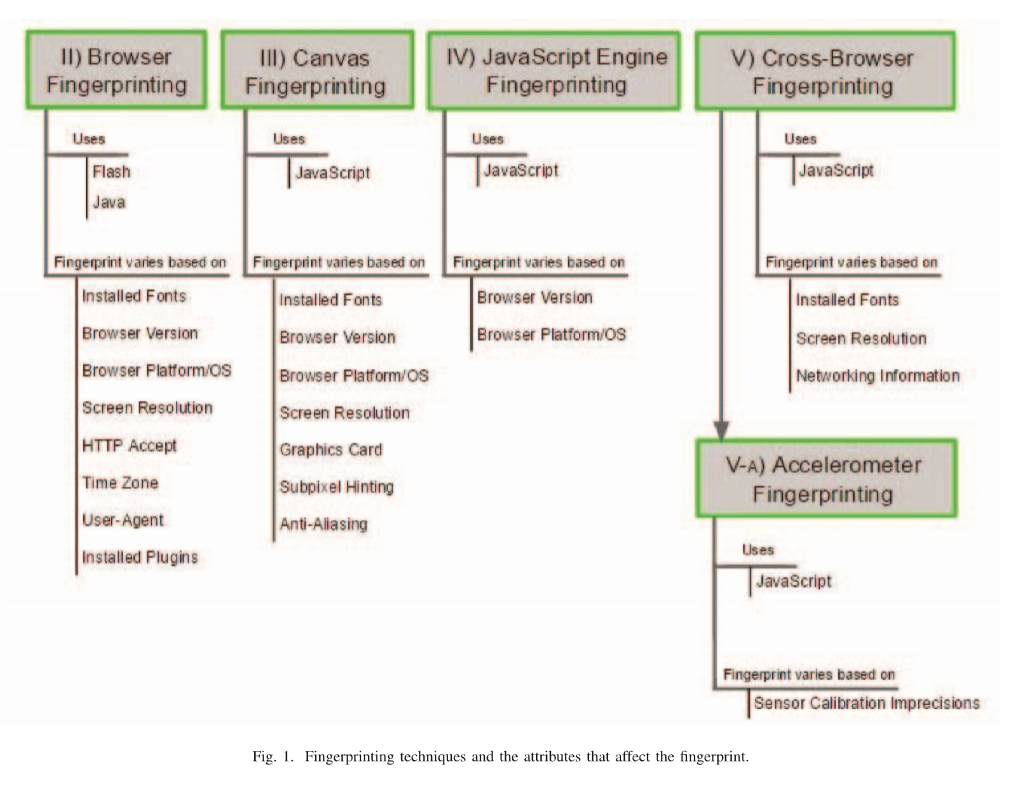
\includegraphics[width=350pt, height=160pt]{FingerprintingAttributes.png}
	\caption{Fingerprinting techniques and the attributes that effect the fingerprint}
	\label{BrowserSpecification}
\end{figure}
\subsection{Browser specific fingerprinting}
%
% more info!
%
* Large scale browser fingerprinting study conducted by P. Eckersley in the Panopticlick project
* has shown 94,2\% of the user with flash or java could be distringuided (without cookies)
* Browser-dependent features (flash/java) to retrieve information on installed fonts, plug-ins, browser platform, screen resolution
* Study showed: only 15-20 bits of identifying info necessary to uniquely identify a particular browser
* most identifying metrics – plug-ins, fonts, user agent, http accept, screen resolution – plug-ins due to version numbers
(\textcite{upi15}, p.2)

Weaknesses: (\textcite{upi15}, p.2)
\begin{itemize}
	\item unable to distinguish between instances of identically configured devices
	\item fingerprint can change across browsers
	\item fingerprint can be easily changed (upgrade, plug-in, etc.)
\end{itemize}
* fp easily changed through upgrades, new installed features or external change of the system 
* -> heuristics which can be used to adapt the fingerprint.  (\textcite{upi15}, p.2)

There are 17 features presented in the Table I of the AmIUnique paper,
and we have all of them for our single-browser fingerprinting.
(\textcite{Cao17}, p.2)
--> look AmIUnique

\subsection{Canvas fingerprinting}
Canvas fingerprinting was first mentioned and implemented by Mowery and Shacham in 2012 as part of their work "Pixel Perfect: Fingerprinting Canvas in HTML5".\\
As the title teasers, this web browser fingerprinting technique works by using the new coding features in HTML5.(\textcite{pixel18}) Any website that runs JavaScript on the user's browser can use the HTML5<canvas> element and observe its rendering behaviour. There is no need for any special access to system resources. (\textcite{mowery12}, p.1)(\textcite{upi15}, p.2)\\\\
For rendering text fonts, webfonts were used as they are more distringuishable than expected. (\textcite{mowery12}, p.6) Further WebGL was used as  graphic cards leave a detectable fingerprint while rendering even the simplest scenes.(\textcite{mowery12}, p.8)\\
\begin{tcolorbox}
	Example text rendering: \\
	Out of 300 samples the text font Arial was rendered in 50 distinct ways. (\textcite{mowery12}, p.6)
\end{tcolorbox}
The outcome of their research and tests was that the canvas fingerprint is consistent but would change depending on hardware and software configuration. Further Mowery and Shacham discovered that the canvas fingerprint is unable to distinguish between users who use the exact same hadware and software.(\textcite{mowery12}, p.5)\\\\
Only 2 years after its first use a study conducted by Acar et al.(2014) ascertained that canvas fingerprinting is the most common form of fingerprinting with an approximately occurrence of 5.5\% in the top 100,000 websites. (\textcite{upi15}, p.2)

\subsubsection{Weaknesses}
(\textcite{upi15}, p.2)
\begin{itemize}
	\item unable to distinguish between instances of identically configured devices
	\item fingerprint can change across browsers
\end{itemize}

\subsubsection{How it works}
Canvas fingerprinting renders text and WebGL scenes onto an area of the screen using the HTML5<canvas> element programmatically and reads the pixel data back to generate a fingerprint. Through this process a 2D graphic context is obtained and a text or image is drawn to the canvas.(\textcite{upi15}, p.2)\\
The obtained canvas object provides a to-DataUrl(type) method which gives a data url consisting of a Base64 encoding of a png image which contains the canvas' contents. This Base 64 encoded pixel data url is used to create a hash.(\textcite{mowery12}, p.3)(\textcite{upi15}, p.2)\\\\
At least the operating system, browser version, graphics card, installed fonts, sub-pixel hinting and anti-aliasing all play a part in the final fingerprint.(\textcite{upi15}, p.2) \\\\
In their thesis K. Mowery and H. Shacham used two types of image comparisons: pixel-level difference and difference maps.(\textcite{mowery12}, pp.4)\\\\
Pixel-level difference works by setting each pixel's color to a channel-wise difference between tow images at that location. If the color is something else thatn transparent pure black it indicates that there is a difference between the two pixels. They set the alpha value of differing pixel to 255 to render it completly opaque. (\textcite{mowery12}, pp.4)\\\\
Difference maps works in a similar way, only that this method sets a pixel either black or white, depending on if they differ. If an image is purely white it indicates that they are the identical image. (\textcite{mowery12}, pp.4)

%It is transparent to the user. Our tests can be performed, offscreen, in a fraction of a second. There is no indication, visual or otherwise, that the user’s system is being fingerprinted.

%entropy
%* Overall, our fingerprints do combine beneficially: 
%* among the 116 groups, our five extremely simple tests show a distribution entropy of 5.73 bits. We believe that more specialized and targeted tests could reveal even more, perhaps down to the exact installed graphics card, operating system, and browser family. (\textcite{mowery12}, p.8)

%* It is high-entropy. In 294 experiments on Amazon’s Mechanical Turk, we observed 116 unique fingerprint values, for a sample entropy of 5.73 bits. This is so even though the user population in our experiments exhibits little variation in browser and OS. (\textcite{mowery12}, p.1)

%When writing their thesis Mowery et al. did not have access to various hundreds distrinct customer-level computer systems and therefore went to use Amazon Mechanical Turk and were able to collect samples from 300 distrinct member of this marketplace.(\textcite{mowery12}, pp.4) Running 5 fingerprinting tests in the background they collected metadata (browser's user agent string, WebGL-reported renderer, vendor, and version.
 
\subsection{JavaScript Engine fingerprinting}

In 2011 P. Reischl et al. published their first paper about the use of the JavaScript Engine to uniquely identify a web browser and major version. Comparing it to the Panopticlick project (\textcite{eckersley10}) it was stated in the paper that the new approach is multiple times faster and error prone. (\textcite{reschl11}, p.2) Two years later, in 2013, the same team with some additional authors published another paper in which this fingerprint technique was described in more detail.(\textcite{mulazzani13}, p.1) \\\\
JavaScript Engine fingerprinting uses testsuits like Sputnik to determine the used browser and version. Compared to other methods this technique does not rely on the user agent string (which can be modified, see \autoref{UAS}) which makes it a more robost fingerprinting technique.(\textcite{mulazzani13}, p.1)

\subsubsection{How it works}
JavaScript Engine fingerprinting works by running test cases of conformance tests like Sputnik and test 262 to identify browsers and their major versions. Even though these test suits consist of multiple thousands test cases the browser only needs to fail one particular test which every other browser passed to be identified. Therefore these fingerprinting technique only needs a fraction of a second to be executed. (\textcite{mulazzani13}, p.3) \\\\
There are two methods which can be used to identify the webbrowser and the major version.\\\\
For a rather small test set the minimal fingerprint method can be used. First test262 is started for each browser in the set and the results are compared. For each browser a test is selected which only this specific browser failed. They select a test case which only one browser failed. This browser can be uniquely identified by this test and is therefore removed from the set. This process is redone for each browser until there is a unique fingerprint for each browser in the set or there is no test case which only one browser failed. If there is no unique fingerprint for a browser the selection is simply changed.(\textcite{mulazzani13}, p.3)\\\\
The figure below shows how the uniqueness of browsers and tests is obtained. The check marks mean, that the respective browser has passed the test. Each test which has a uniqueness of 1 can be used to uniquely identify a browser.
\begin{figure}[H]
	\centering
	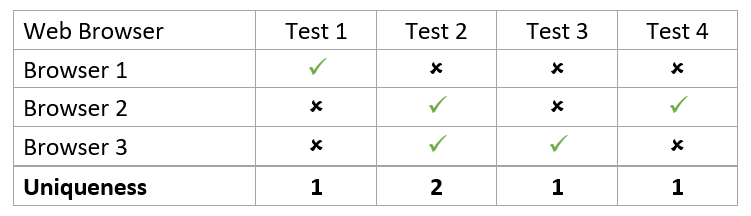
\includegraphics[width=350pt, height=100pt]{MinimalFP.png}
	\caption{Example for the structure of a minimal fingerprint}
	\label{MinimalFP}
\end{figure}
If the test set is rather large it is more effective to use a binary decision tree. This method runs multiple test rounds to determine a web browser and major version. There is no need for a unique fingerprint as the tests split the browsers to identify them. Therefore there is no need to run a test for each browser and version like the  minimal fingerprint would which reduces the total number of executed tests. (\textcite{mulazzani13}, p.4)\\\\
The figure below \textbf{reference} give a good overview how such a tree can be structured. The leaf nodes pose as browsers, the inner nodes display the used tests and the edges indicate the success. (\textcite{mulazzani13}, p.4)
\begin{figure}[H]
	\centering
	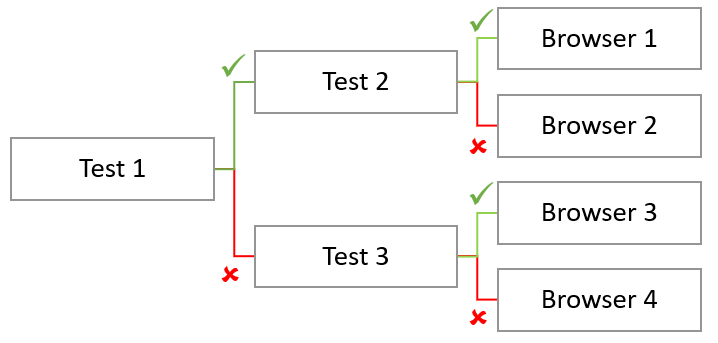
\includegraphics[width=340pt, height=150pt]{DecisionTree.png}
	\caption{Example for the structure of a decision tree}
	\label{DecisionTree}
\end{figure}

\begin{comment}
--  having a comparable overhead for creating and collecting fingerprint samples.
-- implemented in just a few hundred lines of JS
-- undetectable for the user - CPU not stalled noticeably
(\textcite{mulazzani13}, p.2)
-- used to detect modified User-Agent strings, and can be used to reliably identify the browser of Tor Browser Bundle users.
(\textcite{upi15}, p.2)
\end{comment}
\subsection{Cross-Browser fingerprinting}

different kinds of cross-browser finger printing - first by boda - using ip - not so good
in 2017 cao proposes- better option

-- uses browser-independent features for the fingerprint
-- can rely solely on js and use font detection as a techniue
-- since a js engine is available and enabled by default on all modern browsers 
-- differs form techniques which rely on browser dependent plug-ins Adobe Flash or Java for obtaining a font list
(\textcite{upi15}, pp.2)
 
Weaknesses: (\textcite{upi15}, pp.2)
\begin{itemize}
	\item unable to distinguish between instances of identically configured devices
	\item fingerprint can change????
\end{itemize} 
 

A technique developed by Yinzhi Cao
**	New method, created by Yinzhi Cao
**	E.g. used screen’s ratio of width to height as it remains consistent even when using zoom
**	Adapted 4 such features from AmIUnique (which used screen resolution – not consistent)
**	Examination of a user’s audio stack, graphics card, and CPU
**	Relies on 29 features
**	Script forces system to perform 36 tasks – results include info, takes less than a minute
**	Only on Tor it didn’t work
**	(\textcite{nordrum17})

**	Rely on corresponding OS and hardware functionalities
**	99,24\%  successfully identify (\textcite{Cao17})

-- first by boda
-- then extended by cao


(\textcite{boda11})
-- a part of the ip address, availability of a specific font set, time zone, screen resolution
-- uniquely identify most users of the 5 most popular web browsers
-- user agent strings - effective but fragile identifiers of browser instance
(\textcite{boda11}, p.1)

-- browser-independent features as a basis of identification
-- eg. networking information (ip address, hostname, tcp port number)
-- eg. application layer information (uas in http header, name/version of os, extemsions, etc.)
-- eg. info gained by querying - over js - list of fonts, plugins(+version), screen resolution, time zone
(\textcite{boda11}, p.2)

--create a unique identifier from specific browser data using JavaScript and server-side algorithms
(\textcite{boda11}, p.4)

-- crossdomain tracking is achieved by using only the first two octets of the IP address, which
remains constant in many cases even if the IP address of the client changes dynamically
-- may change after switching to a different ISP or another service
-- use locality, short user id(script-generated identifier, derived from the first two octets of the IP address), usa, os, screen, timezone, basic fonts, all fonts, browser name and version
(\textcite{boda11}, p.5)

-- font lists provide a solid base for unique identification under the Windows and Mac OSes
(\textcite{boda11}, p.8)

 The latter is true largely due to the fact that the list
of fonts is easily accessible through the JavaScript API. Therefore, if resistance of
identification is to be secured with the web browsers of today, the only option seems
to be to disable such scripts. That way, one’s anonymity set can be greatly increased.
Users of computers in a set of identically configured machines are likely to have
the best odds against our fingerprinting algorithm. If such computers are centrally
managed, it is unlikely that any of them has a unique feature based on which it could
be identified. Therefore, passive methods are insufficient in such a context.
Our research has some important implications regarding the user’s behaviour. We
have provided recommendations about browser types and versions that are likely
indistinguishable from other such browsers. Furthermore, it can be seen that
resistance to identification is easier achieved with popular system settings. It must be
noted, however, that these measures are not necessarily easy to carry out without
causing inconvenience to the user.
We have also given some guidelines for developers to make their browsers resist
our fingerprinting algorithm. In particular, the verbosity of the UAS and the plugin
versions should be decreased, and a standard ‘substitute font set’ – preferably
supported by all browsers – should be introduced. Furthermore, users should be able
to set fake system properties in the browser in order to hide their real operating
system, time zone and screen resolution.
Finally, we have proposed some improvements for our method, and defined certain
directions for future experiments; an explicitly cross-browser experiment would
provide a high-precision dataset. 
(\textcite{boda11}, p.16)
unavailable behind an anonymous network or a proxy (\textcite{Cao17}, p.1)



-- based on many novel OS and hardware level features, e.g.,
these from graphics card, CPU, audio stack, and installed
writing scripts. Specifically, because many of such OS and
hardware level functions are exposed to JavaScript via browser
APIs, we can extract features when asking the browser to perform
certain tasks through these APIs. The extracted features
can be used for both single- and cross-browser fingerprinting.

(\textcite{Cao17}, p.1)

-- use many novel OS and hardware features, especially computer graphics ones
-- successfully fingerprint 99.24\% of users
-- 83.24\% uniqueness with 91.44\% cross-browser stability
-- Boda excluding IP address only have 68.98\% uniqueness with 84.64\% cross-browser stability.
--  current measurement of screen resolution, e.g.AmIUnique, Panopticlick, Boda - unstable
-- resolution changes in Firefox and IE when zooms
-- zoom level into consideration, normalize the width and height in screen resolution
-- DataURL and JPEG formats are unstable across different browsers, because these formats are with loss and implemented differently in multiple browsers and the server side as well.
-- need to adopt lossless formats for server-client communications in cross-browser fingerprinting.
-- use PNG, a lossless format, for cross-browser fp
-- Prior Fingerprintable Features
-- 4 features for cross-browser fp (screen res., color depth, list of fonts, platform)
-- nr of CPU virtual cores
-- screen resolution (in js simply "screen") - firefox/ie - change resolution value according to zoom level
-- use zoom levels, adjust resolution, screen ration also important
(\textcite{Cao17}, p.2)

-- nr of CPU virtual cores - obtained by browser feature "hardwareConcurrency"
-- audiocontext - provides bundle of audio signal processing functionalities from signal generation to signal
--peak values and their corresponding frequencies are relatively stable
across browsers. 
-- create a list of bins with small steps on both the frequency and value axes, and map the peak
frequencies and values to the corresponding bins.
-- If one bin contains a frequency or value, we mark the bin as one and
otherwise zero: such list of bins serve as our cross-browser feature.
-- List of Fonts width and height of a certain string is measured to determine font type
-- Line, curve, and anti-aliasing. Line and curve are 2D features
supported by both Canvas (2D part) and WebGL.
--Vertex shader. A vertex shader, rendered by GPU and the
driver, converts each vertex in a 3D model to its coordinate in
a 2D clip-space.
-- Fragment shader. A fragment shader, rendered by GPU and
the driver as well, processes a fragment, such as a triangle
outputted by the rasterization, into a set of colors and a single
depth value.
--- MANY MORE - not write down all, als need to cut short - max. 1page per technique!!!!
(\textcite{Cao17}, p.3)

HOW it works:
-- task manager at server side - send various randering tasks
-- e.g. drawing curves, lines to client side
-- rendering task - also obtaining OS and hw level info
-- client-side browser renders and produces results (images, sound waves)
-- results convert into hashes -> to send to server
-- meantime - browser collect browser-specific info (for fp composition)
-- fp is generated from list of hashes from client side and a mask
-- that is a list of 1 or 0 corresponding to the hash list
-- perform "and" operation between list of hashes and mask -> create another hash as fp
-- mask: if browser not support anti-aliasing - all bit in mask involve anti-alisaing -> 0
-- second part of mask -> each browser pair - different mask
(\textcite{Cao17}, p.4)

-- add rendering task? p-5

FP composition
-- how to make fp on server side from client-side hashes
-- computed with -and- operation
-- generation of mask for every two browsers is training-based approach
(\textcite{Cao17}, p.7)

-- go through results?

-- tor browser -> many features unavailable
-- disables canvas by default -> not fingerprintables if disabled?
(\textcite{Cao17}, p.13)